\documentclass[tikz,border=8pt]{standalone}
\usepackage{xcolor}
\usetikzlibrary{arrows.meta,positioning}
\tikzset{
  stage/.style={
    draw,
    rounded corners=5pt,
    minimum width=3.25cm,
    minimum height=2.45cm,
    text width=3.0cm,
    align=center,
    font=\small,
    line width=0.9pt
  },
  flow/.style={->, >=Latex, thick, draw=gray!70}
}
\begin{document}
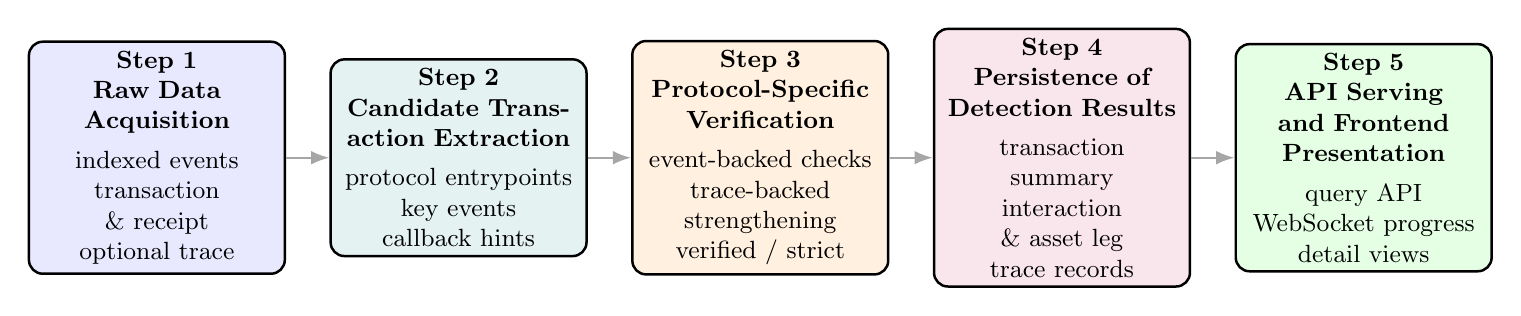
\begin{tikzpicture}[node distance=0.55cm]
  \node[stage, fill=blue!9] (s1) {\textbf{Step 1}\\\textbf{Raw Data Acquisition}\\[0.35em]indexed events\\transaction \& receipt\\optional trace};
  \node[stage, fill=teal!10, right=of s1] (s2) {\textbf{Step 2}\\\textbf{Candidate Transaction Extraction}\\[0.35em]protocol entrypoints\\key events\\callback hints};
  \node[stage, fill=orange!12, right=of s2] (s3) {\textbf{Step 3}\\\textbf{Protocol-Specific Verification}\\[0.35em]event-backed checks\\trace-backed strengthening\\verified / strict};
  \node[stage, fill=purple!10, right=of s3] (s4) {\textbf{Step 4}\\\textbf{Persistence of Detection Results}\\[0.35em]transaction summary\\interaction \& asset leg\\trace records};
  \node[stage, fill=green!10, right=of s4] (s5) {\textbf{Step 5}\\\textbf{API Serving and Frontend Presentation}\\[0.35em]query API\\WebSocket progress\\detail views};

  \draw[flow] (s1) -- (s2);
  \draw[flow] (s2) -- (s3);
  \draw[flow] (s3) -- (s4);
  \draw[flow] (s4) -- (s5);
\end{tikzpicture}
\end{document}
